% ! Tex program = xelatex
\documentclass{article}
\usepackage{pst-node}
% 中文
% \usepackage[UTF8]{ctex}

% For more choices
% %! Tex program = xelatex
% \documentclass{article}
%中文
%\usepackage[UTF8]{ctex}
%数学公式
\usepackage{amsmath,amssymb}
%\usepackage{ntheorem}
% \usepackage[framemethod=TikZ]{mdframed}
\usepackage{amsthm}
%边界
\usepackage[letterpaper,top=3cm,bottom=3cm,left=2cm,right=2cm,marginparwidth=1.75cm]{geometry}%table package
%Table
\usepackage{multirow,booktabs}
\usepackage{makecell}
%字体颜色
\usepackage{color}
\usepackage[dvipsnames]{xcolor}  % 更全的色系
%代码
\usepackage[OT1]{fontenc}
% MATLAB 代码风格
% \usepackage[framed,numbered,autolinebreaks,useliterate]{/Users/anye_zhenhaoyu/Desktop/Latex/mcode}
\usepackage{listings}
\usepackage{algorithm}
\usepackage{algorithmic}
\usepackage{pythonhighlight} % Python
%插图
\usepackage{graphicx}
%改变item格式
\usepackage{enumerate}
%物理
\usepackage{physics}
%extra arrows
\usepackage{extarrows}
% caption(居中指令)
\usepackage[justification=centering]{caption}
% \usepackage{caption}
% htpb
\usepackage{stfloats}
% pdf 拼接
\usepackage{pdfpages}
% 超链接url
\usepackage{url}
% \usepackage{tikz}
\usepackage{pgfplots}
\pgfplotsset{compat=newest}
\usepackage[colorlinks=true, allcolors=blue]{hyperref}
\usepackage{setspace}

% --------------definations-------------- %
\def\*#1{\boldsymbol{#1}}
\def\+#1{\mathcal{#1}} 
\def\-#1{\bar{#1}}
% Domains
\def\RR{\mathbb{R}}
\def\CC{\mathbb{C}}
\def\NN{\mathbb{N}}
\def\ZZ{\mathbb{Z}}
% Newcommand
\newcommand{\inner}[2]{\langle #1,#2\rangle} 
\newcommand{\numP}{\#\mathbf{P}} 
\renewcommand{\P}{\mathbf{P}}
\newcommand{\Var}[2][]{\mathbf{Var}_{#1}\left[#2\right]}
\newcommand{\E}[2][]{\mathbf{E}_{#1}\left[#2\right]}
\renewcommand{\emptyset}{\varnothing}
\newcommand{\ol}{\overline}
\newcommand{\argmin}{\mathop{\arg\min}}
\newcommand{\argmax}{\mathop{\arg\max}}
\renewcommand{\abs}[1]{\qty|#1|}
\newcommand{\defeq}{\triangleq} % triangle over =
\def\deq{\xlongequal{def}} % 'def' over =
\def\LHS{\text{LHS}}
\def\RHS{\text{RHS}}
\def\angbr#1{\langle#1\rangle} % <x>

\def\Esolve{\textcolor{blue}{Solve: }}
\def\Eproof{\textcolor{blue}{Proof: }}
\def\case#1{\textcolor{blue}{Case \uppercase\expandafter{\romannumeral#1}: }}

\newtheorem{lemma}{Lemma}
\newtheorem{thm}{Theorem}
\newtheorem{defi}{Definition}
\newtheorem{prp}{Proposition}
\newenvironment{md}{\begin{mdframed}}{\end{mdframed}}

\date{\today}
\usepackage{fancyhdr}
\pagestyle{fancy}
\fancyhead[L]{\slshape{Haoyu Zhen}}
\fancyhead[R]{{\today}}

% \begin{document}
% \title{<++>}
\author{Haoyu Zhen}
% \maketitle
\setlength{\parindent}{0pt}
\setstretch{1.2}
% \end{document}


% % theorems
\usepackage{thmtools}
\usepackage{thm-restate}
\usepackage[framemethod=TikZ]{mdframed}
\mdfsetup{skipabove=1em,skipbelow=0em, innertopmargin=12pt, innerbottommargin=8pt}

\theoremstyle{definition}

\declaretheoremstyle[headfont=\bfseries\sffamily, bodyfont=\normalfont,
	mdframed={
		nobreak,
		backgroundcolor=brown!14,
		topline=false,
		rightline=false,
		leftline=true,
		bottomline=false,
		linewidth=2pt,
		linecolor=brown!180,
	}
]{thmbrownbox}

\declaretheoremstyle[headfont=\bfseries\sffamily, bodyfont=\normalfont,
	mdframed={
		nobreak,
		backgroundcolor=Blue!4,
		topline=false,
		rightline=false,
		leftline=true,
		bottomline=false,
		linewidth=2pt,
		linecolor=NavyBlue!120,
	}
]{thmbluebox}

\declaretheoremstyle[headfont=\bfseries\sffamily, bodyfont=\normalfont,
	mdframed={
		nobreak,
		backgroundcolor=Green!5,
		topline=false,
		rightline=false,
		leftline=true,
		bottomline=false,
		linewidth=2pt,
		linecolor=OliveGreen!120,
	}
]{thmgreenbox}

\declaretheoremstyle[headfont=\bfseries\sffamily, bodyfont=\normalfont,
	mdframed={
		nobreak,
		topline=false,
		rightline=false,
		leftline=true,
		bottomline=false,
		linewidth=2pt,
		linecolor=OliveGreen!120,
	}
]{thmgreenline}

\declaretheoremstyle[headfont=\bfseries\sffamily, bodyfont=\normalfont,
	mdframed={
		nobreak,
		topline=false,
		rightline=false,
		leftline=true,
		bottomline=false,
		linewidth=2pt,
		linecolor=NavyBlue!70,
	}
]{thmblueline}

\declaretheorem[numberwithin=section, style=thmbrownbox, name={\color{Brown}Definition}]{defi}
\declaretheorem[numberwithin=section, style=thmgreenbox, name={\color{OliveGreen}Law}]{law}
\declaretheorem[numberwithin=section, style=thmbluebox, name={\color{Blue}Corollary}]{cor}
\declaretheorem[numberwithin=section, style=thmgreenline, name={\color{OliveGreen}Property}]{prt}
\declaretheorem[numberwithin=section, style=thmbluebox, name={\color{Blue}Proposition}]{prp}
\declaretheorem[numberwithin=section, style=thmbluebox, name={\color{Blue}Theorem}]{thm}
\declaretheorem[numberwithin=section, style=thmbluebox, name={\color{Blue}Lemma}]{lemma}
\declaretheorem[numberwithin=section, style=thmbrownbox,  name={\color{Brown}Example}]{eg}
\declaretheorem[numberwithin=section, style=thmgreenline, name={\color{OliveGreen}Remark}]{remark}
\declaretheorem[numbered=no,style=thmblueline, name={\color{NavyBlue!70}Proof},qed=$\square$]{prf}
\numberwithin{equation}{section}


% %! Tex program = xelatex
% \documentclass{article}
%中文
%\usepackage[UTF8]{ctex}
%数学公式
\usepackage{amsmath,amssymb}
%\usepackage{ntheorem}
% \usepackage[framemethod=TikZ]{mdframed}
\usepackage{amsthm}
%边界
\usepackage[letterpaper,top=3cm,bottom=3cm,left=2cm,right=2cm,marginparwidth=1.75cm]{geometry}%table package
%Table
\usepackage{multirow,booktabs}
\usepackage{makecell}
%字体颜色
\usepackage{color}
\usepackage[dvipsnames]{xcolor}  % 更全的色系
%代码
\usepackage[OT1]{fontenc}
% MATLAB 代码风格
% \usepackage[framed,numbered,autolinebreaks,useliterate]{/Users/anye_zhenhaoyu/Desktop/Latex/mcode}
\usepackage{listings}
\usepackage{algorithm}
\usepackage{algorithmic}
\usepackage{pythonhighlight} % Python
%插图
\usepackage{graphicx}
%改变item格式
\usepackage{enumerate}
%物理
\usepackage{physics}
%extra arrows
\usepackage{extarrows}
% caption(居中指令)
\usepackage[justification=centering]{caption}
% \usepackage{caption}
% htpb
\usepackage{stfloats}
% pdf 拼接
\usepackage{pdfpages}
% 超链接url
\usepackage{url}
% \usepackage{tikz}
\usepackage{pgfplots}
\pgfplotsset{compat=newest}
\usepackage[colorlinks=true, allcolors=blue]{hyperref}
\usepackage{setspace}

% --------------definations-------------- %
\def\*#1{\boldsymbol{#1}}
\def\+#1{\mathcal{#1}} 
\def\-#1{\bar{#1}}
% Domains
\def\RR{\mathbb{R}}
\def\CC{\mathbb{C}}
\def\NN{\mathbb{N}}
\def\ZZ{\mathbb{Z}}
% Newcommand
\newcommand{\inner}[2]{\langle #1,#2\rangle} 
\newcommand{\numP}{\#\mathbf{P}} 
\renewcommand{\P}{\mathbf{P}}
\newcommand{\Var}[2][]{\mathbf{Var}_{#1}\left[#2\right]}
\newcommand{\E}[2][]{\mathbf{E}_{#1}\left[#2\right]}
\renewcommand{\emptyset}{\varnothing}
\newcommand{\ol}{\overline}
\newcommand{\argmin}{\mathop{\arg\min}}
\newcommand{\argmax}{\mathop{\arg\max}}
\renewcommand{\abs}[1]{\qty|#1|}
\newcommand{\defeq}{\triangleq} % triangle over =
\def\deq{\xlongequal{def}} % 'def' over =
\def\LHS{\text{LHS}}
\def\RHS{\text{RHS}}
\def\angbr#1{\langle#1\rangle} % <x>

\def\Esolve{\textcolor{blue}{Solve: }}
\def\Eproof{\textcolor{blue}{Proof: }}
\def\case#1{\textcolor{blue}{Case \uppercase\expandafter{\romannumeral#1}: }}

\newtheorem{lemma}{Lemma}
\newtheorem{thm}{Theorem}
\newtheorem{defi}{Definition}
\newtheorem{prp}{Proposition}
\newenvironment{md}{\begin{mdframed}}{\end{mdframed}}

\date{\today}
\usepackage{fancyhdr}
\pagestyle{fancy}
\fancyhead[L]{\slshape{Haoyu Zhen}}
\fancyhead[R]{{\today}}

% \begin{document}
% \title{<++>}
\author{Haoyu Zhen}
% \maketitle
\setlength{\parindent}{0pt}
\setstretch{1.2}
% \end{document}


% % theorems
\usepackage{thmtools}
\usepackage{thm-restate}
\usepackage[framemethod=TikZ]{mdframed}
\mdfsetup{skipabove=1em,skipbelow=0em, innertopmargin=12pt, innerbottommargin=8pt}

\theoremstyle{definition}

\declaretheoremstyle[headfont=\bfseries\sffamily, bodyfont=\normalfont,
	mdframed={
		nobreak,
		backgroundcolor=brown!14,
		topline=false,
		rightline=false,
		leftline=true,
		bottomline=false,
		linewidth=2pt,
		linecolor=brown!180,
	}
]{thmbrownbox}

\declaretheoremstyle[headfont=\bfseries\sffamily, bodyfont=\normalfont,
	mdframed={
		nobreak,
		backgroundcolor=Blue!4,
		topline=false,
		rightline=false,
		leftline=true,
		bottomline=false,
		linewidth=2pt,
		linecolor=NavyBlue!120,
	}
]{thmbluebox}

\declaretheoremstyle[headfont=\bfseries\sffamily, bodyfont=\normalfont,
	mdframed={
		nobreak,
		backgroundcolor=Green!5,
		topline=false,
		rightline=false,
		leftline=true,
		bottomline=false,
		linewidth=2pt,
		linecolor=OliveGreen!120,
	}
]{thmgreenbox}

\declaretheoremstyle[headfont=\bfseries\sffamily, bodyfont=\normalfont,
	mdframed={
		nobreak,
		topline=false,
		rightline=false,
		leftline=true,
		bottomline=false,
		linewidth=2pt,
		linecolor=OliveGreen!120,
	}
]{thmgreenline}

\declaretheoremstyle[headfont=\bfseries\sffamily, bodyfont=\normalfont,
	mdframed={
		nobreak,
		topline=false,
		rightline=false,
		leftline=true,
		bottomline=false,
		linewidth=2pt,
		linecolor=NavyBlue!70,
	}
]{thmblueline}

\declaretheorem[numberwithin=section, style=thmbrownbox, name={\color{Brown}Definition}]{defi}
\declaretheorem[numberwithin=section, style=thmgreenbox, name={\color{OliveGreen}Law}]{law}
\declaretheorem[numberwithin=section, style=thmbluebox, name={\color{Blue}Corollary}]{cor}
\declaretheorem[numberwithin=section, style=thmgreenline, name={\color{OliveGreen}Property}]{prt}
\declaretheorem[numberwithin=section, style=thmbluebox, name={\color{Blue}Proposition}]{prp}
\declaretheorem[numberwithin=section, style=thmbluebox, name={\color{Blue}Theorem}]{thm}
\declaretheorem[numberwithin=section, style=thmbluebox, name={\color{Blue}Lemma}]{lemma}
\declaretheorem[numberwithin=section, style=thmbrownbox,  name={\color{Brown}Example}]{eg}
\declaretheorem[numberwithin=section, style=thmgreenline, name={\color{OliveGreen}Remark}]{remark}
\declaretheorem[numbered=no,style=thmblueline, name={\color{NavyBlue!70}Proof},qed=$\square$]{prf}
\numberwithin{equation}{section}


% On my MAC's Desktop
%! Tex program = xelatex
% \documentclass{article}
%中文
%\usepackage[UTF8]{ctex}
%数学公式
\usepackage{amsmath,amssymb}
%\usepackage{ntheorem}
% \usepackage[framemethod=TikZ]{mdframed}
\usepackage{amsthm}
%边界
\usepackage[letterpaper,top=3cm,bottom=3cm,left=2cm,right=2cm,marginparwidth=1.75cm]{geometry}%table package
%Table
\usepackage{multirow,booktabs}
\usepackage{makecell}
%字体颜色
\usepackage{color}
\usepackage[dvipsnames]{xcolor}  % 更全的色系
%代码
\usepackage[OT1]{fontenc}
% MATLAB 代码风格
% \usepackage[framed,numbered,autolinebreaks,useliterate]{/Users/anye_zhenhaoyu/Desktop/Latex/mcode}
\usepackage{listings}
\usepackage{algorithm}
\usepackage{algorithmic}
\usepackage{pythonhighlight} % Python
%插图
\usepackage{graphicx}
%改变item格式
\usepackage{enumerate}
%物理
\usepackage{physics}
%extra arrows
\usepackage{extarrows}
% caption(居中指令)
\usepackage[justification=centering]{caption}
% \usepackage{caption}
% htpb
\usepackage{stfloats}
% pdf 拼接
\usepackage{pdfpages}
% 超链接url
\usepackage{url}
% \usepackage{tikz}
\usepackage{pgfplots}
\pgfplotsset{compat=newest}
\usepackage[colorlinks=true, allcolors=blue]{hyperref}
\usepackage{setspace}

% --------------definations-------------- %
\def\*#1{\boldsymbol{#1}}
\def\+#1{\mathcal{#1}} 
\def\-#1{\bar{#1}}
% Domains
\def\RR{\mathbb{R}}
\def\CC{\mathbb{C}}
\def\NN{\mathbb{N}}
\def\ZZ{\mathbb{Z}}
% Newcommand
\newcommand{\inner}[2]{\langle #1,#2\rangle} 
\newcommand{\numP}{\#\mathbf{P}} 
\renewcommand{\P}{\mathbf{P}}
\newcommand{\Var}[2][]{\mathbf{Var}_{#1}\left[#2\right]}
\newcommand{\E}[2][]{\mathbf{E}_{#1}\left[#2\right]}
\renewcommand{\emptyset}{\varnothing}
\newcommand{\ol}{\overline}
\newcommand{\argmin}{\mathop{\arg\min}}
\newcommand{\argmax}{\mathop{\arg\max}}
\renewcommand{\abs}[1]{\qty|#1|}
\newcommand{\defeq}{\triangleq} % triangle over =
\def\deq{\xlongequal{def}} % 'def' over =
\def\LHS{\text{LHS}}
\def\RHS{\text{RHS}}
\def\angbr#1{\langle#1\rangle} % <x>

\def\Esolve{\textcolor{blue}{Solve: }}
\def\Eproof{\textcolor{blue}{Proof: }}
\def\case#1{\textcolor{blue}{Case \uppercase\expandafter{\romannumeral#1}: }}

\newtheorem{lemma}{Lemma}
\newtheorem{thm}{Theorem}
\newtheorem{defi}{Definition}
\newtheorem{prp}{Proposition}
\newenvironment{md}{\begin{mdframed}}{\end{mdframed}}

\date{\today}
\usepackage{fancyhdr}
\pagestyle{fancy}
\fancyhead[L]{\slshape{Haoyu Zhen}}
\fancyhead[R]{{\today}}

% \begin{document}
% \title{<++>}
\author{Haoyu Zhen}
% \maketitle
\setlength{\parindent}{0pt}
\setstretch{1.2}
% \end{document}



\graphicspath{{figures/}}

\begin{document}
% \tableofcontents
\title{Homework 2}
\maketitle
\section*{Problem 1}
Let $T(n)$ be the numebr of all the bit operation we have done after  $n$ ADDs, e.g., $T(1)=1,\,T(2)=3$. $C_n\defeq T(n)-T(n-1)$ and $S_k\defeq T(2^k-1)$.
NB: $(2^k-1)_2=\underbrace{11\cdots1}_k$.

Then we have
\[
	S_k=C_{2^{k-1}}+2S_{k-1}=k+2S_{k-1}
\] which entails
\[
	T(2^k-1)=S_k=2^{k+1}-k-2\qand T(2^k)=2^k-1
	.\]
Thus $\forall n\in\set{2^{k-1},\cdots,2^{k}-1}$
\[
	C(1)+C(2)+\cdots+C(n)=T(n)<T(2^k)<4n\Longrightarrow \mathrm{LHS}=n\+O(1)
	.\]
Finally, the amortized cost of ADD is $\+O(1)$.

\section*{Problem 2}
\textbf{(a).}
The counter-example:
\begin{figure}[H]
	\centering
	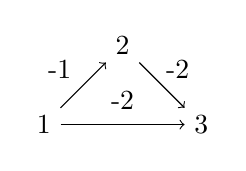
\begin{tikzpicture}
		\node (1) at(0,0) {1};
		\node (2) at(1,1) {2};
		\node (3) at(2,0) {3};
		\draw[->] (1)--(2);
		\draw[->] (2)--(3);
		\draw[->] (1)--(3);
		\node (-1) at(0.2,0.7) {-1};
		\node (-2) at(1,0.3) {-2};
		\node (-3) at(1.7,0.7) {-2};
	\end{tikzpicture}
\end{figure}
The shortest path from 1 to 3 should be:$1\to2\to3$. While this algorithm will return $1\to3$ directly by $(C-2)<(C-1)+(C-2)$ where $C>2$ is the number added to each edge.
\\\\
\textbf{(b).} Worked.

Trivially, $\forall$ path $p$ form $s$ to $v_l$, $p=(s,v_1,v_2,\cdots,v_l)$ where $v_i$ belongs to layer $i$.

Let $p_0=\argmin_p(p \text{ is the shortest path from $s$ to $v_l$})$. Then
\[
	p_0=\argmin_p\qty(l\times C+\sum_{\text{weight $w$ in }p} w)=\argmin_p\qty(\sum_{\text{weight $w$ in }p} w)
\]
where RHS is what we want.

\section*{Problem 3}
\textbf{(a).}
I was inspired by the \textcolor{blue}{Hint} from Chihao Zhang. Let $s$ be the beginning vertex. The algorithm is as follows.

\begin{enumerate}
	\item Construct a graph $H$ having the same topology of  $G$. In $H$, weight $w=rc_{uv}-p_v$ w.r.t. edge $(u,v)$.
	\item Determine if there is a negative loop that $s$ could reach (implement SPFA or Bellman-Ford).
	\item If 2. returns true, then $\exists C$: $\sum_{(u,v)\in C}rc_{uv}-p_v<0$ which means that $r<r^*$. Otherwise $r\ge r^*$.
\end{enumerate}
The complexity is $\+O(\abs{V}\abs{E})$.
\\\\
\textbf{(b).}
For simplicy, ALG.a denotes the algorithm demonstrated in (a).

\begin{algorithm}[H]
	\caption{Find the cycle which has a good profit-to-cost ratio in the given graph}
	\label{fc}
	\begin{algorithmic}
		\renewcommand{\algorithmicrequire}{\textbf{Input:}}
		\renewcommand{\algorithmicensure}{\textbf{Output:}}
		\REQUIRE A graph $G$
		\ENSURE A good enough cycle $C$.
		\STATE $left\gets 0$, $right\gets R$.
		\WHILE{$right-left>\varepsilon$}
		\STATE $r\gets\flatfrac{(right+left)}{2}$ 
		\STATE Implement ALG.a with the input: ratio $r$ and graph  $G$
		\IF{$r>r^*$}
		\STATE $left\gets r$
		\ELSE
			\STATE $right\gets r$
		\ENDIF
		\ENDWHILE
		\STATE Construct the graph $H$ following the rules shown in (a). step 1 with $r=left$
		\IF{$H$ dose not has a negative loop (Under this case, $left = r^*$.)}
		\STATE We could reconstruct the graph  $H$ with $r=left-\flatfrac{\varepsilon}{2}$
		\ENDIF
		\STATE Find a negative loop $C$ in $H$ contained $s$ by Bellman-Ford (More details are in Appendix ALG.\ref{fn})
		\RETURN $C$
	\end{algorithmic} 
\end{algorithm}
Soundness of ALG.\ref{fc}: Obviously, $\forall left,\,right:$ $left\le r^*\le right$. When the ``while'' operation ends, we have $r^*-\varepsilon\le left\le r^*$.
Thus
\[
	\sum_{(u,v)\in C}\qty(left\times c_{uv}-p_v)\le 0
	\Longrightarrow
	r^*-\varepsilon\le left\le r(C)
.\]
The complexity of ALG.\ref{fc}: 
\[
	T(\abs{V},\varepsilon,R)
	=
	\+O\qty[\abs{V}\abs{E}\log_2\qty(\frac{R}{\varepsilon})]
	=
	\+O\qty[\abs{V}^3\log\qty(\frac{R}{\varepsilon})]
.\] 
\newpage
\section*{Problem 4}
\textbf{(a).} Trivially, G only has 2 vertices. $G$: $1--2$ and $G'$:  $1\longrightarrow 2$
\\\\
\textbf{(b).}
% First we define $A_{u}=\set{u}\cup\set{u\text{'s ancestor in $G'$}}$ and $D_{u}=\set{u}\cup\set{u\text{'s descendant in $G'$}}$. Also $G=(V_G,E_G)$ and  $G'=(V_{G'},E_{G'})$.
In $G$, we want to generate 2 paths $p_1$ and $p_2$ such that they share no edge, i.e., $\forall (u_1,v_1)$ in $p_1$ and $(u_2,v_2)$ in $p_2$, $(u_1,v_1)\ne (u_2,v_2)$. We do it by following steps:
\begin{enumerate}
	\item 
		In $G'$, there exist 2 paths $p_1$: $u\to v$ and $p_2$: $v\to u$.
	\item
		If $p_1$, $p_2$ have the same edge $(u',v')$, go to step.3.
	\item
		Assume that $p_1=(u\Rightarrow u'\to \Rnode{tov}{\underline{v'\Rightarrow v}})$ and $p_2=(\Rnode{vu}{\underline{v\Rightarrow u'}}\to v'\Rightarrow u)$ where $a\to b$ implies $a,b$ are adjacent and $a\Rightarrow b$ represents a path from a to b.
	\item Then update:
		$p_1=(u\Rightarrow \Rnode{uv}{\underline{u'\Rightarrow v}})$ and 
		$p_2=(\Rnode{vto}{\underline{v\Rightarrow v'}}\Rightarrow u)$.
		Here $u'\Rightarrow v$ is the inverse of $v\Rightarrow u'$ and $v\Rightarrow v'$ is the inverse of  $v'\Rightarrow v$.
	\item Repeat step 2 until $p_1$ and $p_2$ share no edge.
\end{enumerate}
\ncarc[arrows = ->, linecolor =blue, arcangle = -10, nodesep = 1pt]{vu}{uv}
\ncarc[arrows = ->, linecolor =red, arcangle = -20, nodesep = 1pt]{tov}{vto}
Trivially, $p_1$ and $p_2$ is what we want. Thus, forall $u,v$ in $V$, there are 2 paths from $u$ to $v$ and they share no edge in $G$ $\implies$ removing any single edge from $G$ will still give a connected graph.
\\\\
\textbf{(c).}
From a root $r$ we get a tree $T$ generated by DFS.
\begin{lemma}
	\label{ct}
	Suppose that a vertex $u$ has several subtrees $T_1,T_2,\cdots,T_k$. And we define: $T_i$ is strongly connected in $G$ if $\forall u,v\in$, $u$ could reach $v$ and $v$ could reach $u$ in $G$. Then:
	\[
		\forall i,\,T_i\text{ is strongly connected in }G
		\implies
		T_u\text{ is strongly connected in }G
	\] where $T_u$ is the $G$'s subtree with root $u$.
\end{lemma}
\begin{proof}
	We only need to prove $\forall i$, $\exists$ vertex $v$ in $T_i$, $(v,u')$ is a back edge in $E$ where $u'$ is the ancestor of $u$ or  $u=u'$.
	If not, assume $T_j$ does not satisfy this property. Then we cut the edge ``$e$'' from u to $T_j$.
	Noe we use the property of tree generated by DFS: ``if $(v_1,u_1)\in E$ where $v_1$ is in $T_j$ and $u_1$ is not in, then $u_1$ is the ancestor of $T_j$.''
	Now we have there is no edge from $T_j$ to $u$. Contradiction.
\end{proof}
Here we use induction:

every leaf is strongly connected in $G$. Then by lemma.\ref{ct}, the whole ``tree'' is connected in $G$, which means $G'$ is strongly connected.
\\\\
\textbf{(d).}
Assume that $G$ is connected (or it is trivial).
we design the algorithm intuitively,
\begin{enumerate}
	\item $n\gets 0$
	\item Generate $G'$ through the given rule. (Easy to implement)
	\item Analyse $G'$ using algorithm in ``Slide-06 Page $\S127$ Super Plan'' to find all SCCs 
	\item For every $(u,v)\in E_{G'}$, if $u,v$ belong to different SCCs, then $n\gets n+1$
\end{enumerate}
The correctness of this algorithm holds naturaly because SCCs in Step.2 is a tree which only has tree edges and back edges.

The complexity is $\+O(\abs{V}+\abs{E})$.

\section*{Problem 5}
Get the smallest number $n$ by the following steps:
\begin{enumerate}
	\item Find all the SCCs in $G$, regard every of them as a node and keep the edges between different SCCs. Then we get a DAG: $G'$. 
	\item Separate $G'$ into $k$ isolated component $C_1,C_2,\cdots,C_k$ such that there is no edges between different components and $C_i$ is weakly connected.
	\item $T_i\defeq\text{number of tail vertex in }C_i$ and $H_i\defeq\text{number of head vertex in }C_i$.
	\item $n=k-1+\sum_{i=1}^k\max(T_i,H_i)$.
\end{enumerate}
Reference: \href{https://stackoverflow.com/questions/12681785}{Question.12681785, StackOverflow}.

\section*{Problem 6}
About 15 hours. Difficulty 4. Talked with Yilin Sun and Wei Jiang.

\section*{Appendix}
	How to find a negative loop in graph $H$? Here's the algorithm:
	\begin{algorithm}[H]
	\caption{Find the cycle which has a negative loop in the given graph}
	\label{fn}
	\begin{algorithmic}
		\STATE Implement Bellman-Ford algorithm, during which we record the parents for every updated vertex.
		\STATE In Bellman-Ford algorithm, vertex $v$ has been traversed for  $\abs{V}$ times. 
		\STATE Initiate an array: $\set{a_i}\gets 0$.
		\WHILE{$\forall i$, $a_i\le 1$}
		\STATE $a_v\gets a_v+1$
		\STATE $v\gets v\text{'s parent}$
		\ENDWHILE
		\STATE Suppose that $a_t=2$
		\RETURN $(t,\, t\text{'s parent},\,\cdots,\,t)$
	\end{algorithmic} 
\end{algorithm}
\end{document}
